% =========================================================================
% CHAPTER 8 — EVALUATE: THE USER STUDY
% =========================================================================

\chapter{User Study}
\label{ch:userstudy}

\noindent
{\rmfamily\itshape
\begin{tabular}[t]{@{}l@{\hspace{0.3cm}}p{12.5cm}@{}}
\textls[50]{\textbf{Addressed:}} &
\textls[50]{Testing · Survey · Written comprehension protocol}
\end{tabular}
}

\vspace{0.5cm}

Chapter~\ref{ch:translate} developed the artefact and showed that the two conditions contain the same information. The next question is whether presenting this information in different ways affects how people understand it. This chapter describes the user study designed to investigate this question. The study does not aim to prove that experiential visualisation is better. Instead, it examines whether a small group of mosty non-specialist participants understands the system differently when presented with a static or an experiential visualisation. The study is also designed so that both positive and negative results can provide useful information for the next stage of the research. It is a socio-cognitive study, aimed at understanding how people interpret the visualisations rather than at testing the underlying science or competence of the participants.

% -------------------------------------------------------------------------
\section{Purpose}
\label{sec:eval-purpose}

The central research question asks to what extent machine-learning-driven experiential visualisations improve the cognitive understanding of complex climate tipping systems among non-specialist audiences, compared with conventional static visualisations. Chapters~\ref{ch:data_pipeline} and~\ref{ch:translate} addressed the detection and translation stages of the research. The remaining step was to expose participants to the two forms of representation and compare how they understand them.

A comparative user study is therefore needed to test whether the different visual forms lead to different levels of understanding. Previous research has shown that animated visualisations can appear more effective than static ones, but this can also happen when the animated version contains information that is not available in the static version \citep{tversky2002}. For this reason, the present study keeps the underlying information consistent between the two conditions and changes mainly how that information is presented. The aim is to observe how participants interpret each representation and how experiential ways of presenting information may support deep understanding of complex systems.

% -------------------------------------------------------------------------
\section{An Exploratory First Stage}
\label{sec:eval-exploratory}

The study is exploratory by design. Twenty-five participants took part: twelve were assigned to the static condition and thirteen to the experiential condition. A sample of this size is not sufficient for broad inferential statistics or population-level generalization, and the study does not make such claims.\footnote{The difference between twelve and thirteen participants is a result of random assignment at a small sample size. It does not affect the descriptive analysis, apart from the denominators used when reporting the results in Chapter~\ref{ch:results}.}

The purpose of this first study is instead to identify initial patterns that can inform future research. It can show which concepts participants understand, which concepts are commonly misunderstood, and whether the two visualisation conditions appear to lead to different interpretations. It can also indicate whether the approach is promising enough to justify a larger and statistically powered study.

The study should therefore be understood as a first empirical step rather than as a final test of the proposed approach.

% -------------------------------------------------------------------------
\section{Participants and Audience}
\label{sec:eval-audience}

The study targeted random people, mostly non-specialists: participants without specific training in oceanography, climate science, mathematics or machine learning. This choice directly reflects the aim of the thesis. The visualisations are intended to support the understanding of complex systems beyond specialised scientific audiences.

Participants were not expected to have any prior knowledge of the chosen case study (AMOC) or of the concepts used in the visualisations. The survey provided the basic information needed to approach the scenes.\footnote{Participants were recruited through personal networks in Italian and English. The resulting sample is therefore a convenience sample. Its demographic composition is described in \S\ref{sec:eval-demographics}, while the implications of the sample are discussed in \S\ref{sec:eval-limitations}.}

This is an important part of the study design. If a visualisation can only be understood by people who already know the system, it does not fully address the communication problem considered in this thesis.

% -------------------------------------------------------------------------
\section{The Instrument}
\label{sec:eval-instrument}

Due to its exploratory nature, the study was conducted as a self-guided written survey using Google Forms. Four versions of the survey were used, combining two languages (Italian and English) with the two experimental conditions (static and experiential).\footnote{The four forms use the same wording within each language and differ only in the scene links leading to the static or experiential visualisations. The complete survey protocols are provided in Appendix~\ref{app:protocols}.}

An earlier version of the study considered a think-aloud protocol with live sessions. This approach was later replaced by a written, self-administered survey. The written format makes it possible to reach more participants and gives everyone the same instructions and questions without the presence of an interviewer influencing their responses. This was considered more appropriate for the exploratory study and its relatively small sample.

The survey follows a single sequence. It begins with an introduction to the study, followed by consent, information about anonymity and a short background section. Participants are then given the basic context needed to understand the AMOC and the unit Sverdrup. This information is provided to both groups before they begin the visualisation tasks.

The three scenes then follow:

\begin{enumerate}
    \item \textit{The Column}
    \item \textit{The Engine Room}
    \item \textit{The Threshold}
\end{enumerate}

For each scene, participants first receive a short introduction and a guiding question. They then open the assigned visualisation in a new tab and explore it. After returning to the survey, they answer a series of open questions in their own words.

The survey ends with a final reflection and a debrief. The order of the questions is intentional: participants first describe what they understood in their own words before being asked to rate their confidence or reflect on the experience. The full structure of the study is only explained after the main responses have been collected.

% -------------------------------------------------------------------------
\section{Conditions of the Study}
\label{sec:eval-conditions}

The main difference between the two groups was the type of visualisation they experienced. Both groups saw the same three scenes --- \textit{The Column}, \textit{The Engine Room} and \textit{The Threshold} --- and were given the same underlying questions and contextual information.

The control group saw each scene as a conventional static visualisation. The experiential group saw the corresponding interactive and dynamic version.\footnote{The design of the three scenes and the distinction between their machine-learning-derived and classical components are described in \S\ref{sec:three-scenes}.}

The comparison therefore focuses on the way the information is presented rather than on completely different datasets or scientific content. Chapter~\ref{ch:translate} established that both conditions use the same data bundle, reconstruction function and provenance.

It is also important to clarify that machine learning does not generate every element of the experiential visualisations. Its role differs between scenes, while some elements are based on classical mathematical or visual methods. For example, the particle field in Scene~I is based on a classical derivative, while the ensemble spread in Scene~III comes from external ocean models. The study therefore compares two ways of presenting the same underlying system, rather than simply comparing a machine-learning condition with a non-machine-learning condition. Still, machine learning is a key component of the experiential condition, and the study investigates whether this approach can support a clearer understanding of the system.

% -------------------------------------------------------------------------
\section{Randomisation and the Debrief}
\label{sec:eval-randomisation}

Participants were randomly assigned to one of the two conditions. With a small sample, randomisation cannot guarantee perfectly balanced groups, but it reduces the risk that participants select their own condition and therefore introduces a simple way of limiting systematic selection bias.

Participants remained in their assigned condition until the end of the main study. This was done so that exposure to the alternative visualisation would not influence their responses to the condition being evaluated. The two-condition structure was explained only during the final debrief.\footnote{Keeping the experimental structure undisclosed until the end reduces the possibility that participants interpret their experience as part of a comparison and change their responses accordingly.}

After all main responses had been collected, the debrief explained the study structure and introduced the two conditions. Participants were then given access to the complete set of visualisations, including the version they had not previously experienced.

This final step allows the control group to explore the experiential visualisations as well and gives all participants access to the full set of materials after the study has been completed.

% -------------------------------------------------------------------------
\section{Background Section}
\label{sec:eval-demographics}

A short background section was included before the visualisation tasks. It collected information about age range, education, field of study or work, and self-rated familiarity with climate science, the AMOC and data visualisations.

The purpose of this section is mainly descriptive. Given the small sample size, these variables are not used as a basis for statistical modelling. Instead, they provide information about the participants and help describe the audience included in the study.

The demographic information therefore provides context for the results rather than acting as a separate analytical component.

% -------------------------------------------------------------------------
\section{Consent, Anonymity and Ethics}
\label{sec:eval-ethics}

Participation was voluntary and anonymous. The survey did not collect names, email addresses or other information that could directly identify participants. Participants were informed that they could stop participating at any time without providing a reason.\footnote{The consent text, anonymity statement and image and data disclaimer are reproduced in Appendix~\ref{app:protocols}. Ethics approval for the study was handled through the supervisory process.}

Consent was obtained before the study began through an explicit confirmation that continuing with the survey meant agreeing to participate. The collected responses were used only for the purposes of this research, and no identifying information is included in the analysis or in the results presented in Chapter~\ref{ch:results}.

Because the survey does not collect personal identifiers, the analysis is based only on the responses provided by participants.

% -------------------------------------------------------------------------
\section{Evaluation Framework}
\label{sec:eval-framework}

The open responses are analysed using a predefined coding grid. The aim is not simply to mark answers as right or wrong, but to identify whether participants express the main structural idea represented by each scene.\footnote{The complete coding grid, including the target for each scene and the definition of each category, is provided in Appendix~\ref{app:protocols}.}

The coding categories were defined before analysing the responses. They are linked to the main questions of the three scenes described in \S\ref{sec:three-scenes}. For Scene~I, the main target concerns the existence of opposing directions at different depths. For Scene~II, it concerns the possibility of recurrence between different states. For Scene~III, it concerns changes in the level of agreement between the three models over time.

A response is considered to show understanding of a scene when the participant describes the relevant structure in their own words. Simply mentioning movement, colour or other visual features is not sufficient.

The coding was carried out through an assisted procedure. A large language model, instructed on the coding grid and its category definitions, produced an initial label for each response. The researcher then reviewed every label and corrected it wherever their own judgement differed from the automatic proposal. The final coding is therefore the result of human adjudication, with the automated pass serving only as a starting point.\footnote{The pre-defined coding grid (Appendix~\ref{app:protocols}) is what keeps this procedure transparent: each label can be rechecked by others using the fixed criteria and the original responses. No inter-coder agreement coefficient is reported, as this measure does not apply to a single-coder design supported by an automated first pass. The limitation of single-coder analysis is discussed in \S\ref{sec:eval-limitations}.}

The framework also distinguishes between demonstrated understanding and perceived understanding. Demonstrated understanding is assessed through the participant's written description, while perceived understanding is captured through the participant's confidence rating. These two measures are kept separate because participants may feel confident even when their interpretation does not match the intended structure.\footnote{\textcite{fischer2020} discusses cases in which high confidence can accompany an incorrect interpretation. The present analysis therefore compares confidence with the coded responses rather than treating confidence as evidence of correct understanding.}

This distinction is important because the survey cannot directly measure everything a participant understands. It can only analyse what participants communicate through their responses.

% -------------------------------------------------------------------------
\section{What the Study Expects to Find}
\label{sec:eval-expectations}

The study investigates whether the experiential condition may support a clearer understanding of system behaviour than the static condition.

The expected differences are linked to the three scenes. In Scene~I, the experiential representation may make the relationship between depth and opposing directions easier to understand. In Scene~II, movement may make recurrence between different states easier to recognise. In Scene~III, the dynamic representation may make changes in agreement between the three models easier to perceive over time.

These are expectations rather than confirmed findings. The purpose of the study is to test whether such differences appear in participants' responses. The actual results are presented and discussed in Chapter~\ref{ch:results}.

% -------------------------------------------------------------------------
\section{Timing and Burden}
\label{sec:eval-burden}

The survey was designed to take approximately fifteen to twenty minutes to complete. This was a deliberate choice to keep the study short enough to avoid unnecessary fatigue while still giving participants enough time to explore the three visualisations.

The survey therefore combines a short background section, three visualisation tasks and a final reflection. Participants could stop at any point if they no longer wished to continue.

% -------------------------------------------------------------------------
\section{Limitations of the Design}
\label{sec:eval-limitations}

The study has several important limitations. First, the sample is small, with twenty-five participants in total. The two groups are also slightly unbalanced, with twelve participants in the static condition and thirteen in the experiential condition. The sample size does not provide sufficient statistical power for strong inferential analysis or population-level generalisation.

Second, participants were recruited through personal networks, making the sample one of convenience. Its age, background and experience may therefore differ from those of the wider population that the visualisations are ultimately intended to reach.

Third, the study uses written and self-reported responses. This means that the analysis is limited to what participants are able or willing to express in writing. Some aspects of understanding may therefore remain unobserved.

Fourth, the responses were coded by a single researcher, supported by an automated first pass and without an independent second coder. No inter-coder reliability can therefore be reported. The pre-specified coding grid mitigates this limitation by keeping each assignment open to external rechecking against fixed criteria, but it does not fully replace independent double coding.

Finally, the study distinguishes between demonstrated and perceived understanding. A participant may report high confidence without showing the expected structural understanding in their written response. This is not treated as a methodological error, but as an important distinction that the evaluation framework is designed to capture.

These limitations do not remove the value of the study. The purpose of this work is to provide a first empirical test of the approach and to identify patterns that can guide future research. A larger and more controlled study would be needed to test the findings with greater statistical power. The present study therefore provides an initial empirical foundation rather than a final validation of the proposed approach.

% ============================================================
% fuse* Artificial Botany (2019) -- original figure
% extracted from the studio's website.
% ============================================================

\begin{figure}[htbp]
    \centering
    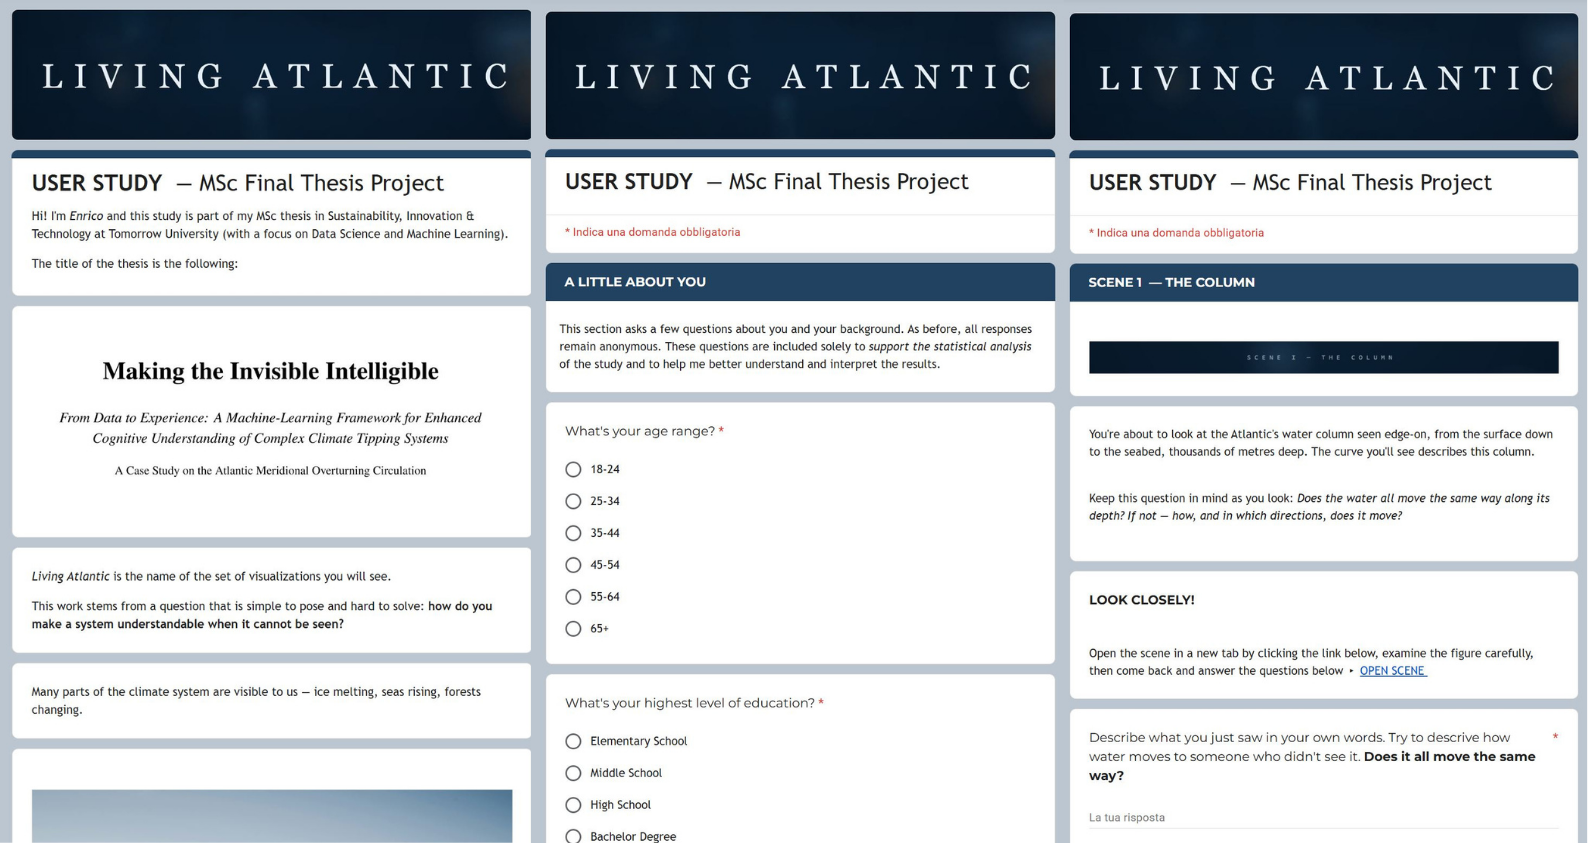
\includegraphics[width=\textwidth]{figures/user_study/Google_Form.png}
    \caption[Google Form]{Google Form used for data collection. The form was designed to collect participants' feedback on the proposed approach, including their experience with the system, perceived usability, and suggestions for improvement.}
    \label{fig:google-form}
\end{figure}